\documentclass{beamer}
%
% Choose how your presentation looks.
%
% For more themes, color themes and font themes, see:
% http://deic.uab.es/~iblanes/beamer_gallery/index_by_theme.html
%
\mode<presentation>
{
  \usetheme{Madrid}      % or try Darmstadt, Madrid, Warsaw, ...
  \usecolortheme{seahorse} % or try albatross, beaver, crane, ...
  \usefonttheme{serif}  % or try serif, structurebold, ...
  \setbeamertemplate{navigation symbols}{}
  \setbeamertemplate{caption}[numbered]
} 

\usepackage[english]{babel}
\usepackage{kotex}
\usepackage{tikz}
\usepackage{listings}
\usepackage{pgffor}
\usepackage{listings}
\usepackage{amsfonts}
\usepackage[linesnumbered,ruled,vlined]{algorithm2e}
\usepackage{algorithmic}

% algorithmbis environment
\makeatletter
\newcounter{algorithmbis}[section]
\setcounter{algorithmbis}{0}
\renewcommand{\thealgorithmbis}{\arabic{algorithmbis}}
\def\algorithmbis{\@ifnextchar[{\@algorithmbisa}{\@algorithmbisb}}
\def\@algorithmbisa[#1]{%
  \refstepcounter{algorithmbis}
  \trivlist
  \leftmargin\z@
  \itemindent\z@
  \labelsep\z@
  \item[\colorbox{lightgray}{\parbox{\textwidth}{%
	    \noindent\strut\textbf{\sf\small 코드 \sf\small\thealgorithmbis} \sf\small#1}
  }]\hfil\vskip0em%
  \color{darkgray}
}
\def\@algorithmbisb{\@algorithmbisa[]}
\def\endalgorithmbis{\hfil\endtrivlist}
\makeatother

\lstset{ %
  backgroundcolor=\color{white},   % choose the background color; you must add \usepackage{color} or \usepackage{xcolor}
  basicstyle=\footnotesize,        % the size of the fonts that are used for the code
  breakatwhitespace=false,         % sets if automatic breaks should only happen at whitespace
  breaklines=true,                 % sets automatic line breaking
  captionpos=b,                    % sets the caption-position to bottom
  commentstyle=\color{gray},    % comment style
  deletekeywords={...},            % if you want to delete keywords from the given language
  escapeinside={\%*}{*)},          % if you want to add LaTeX within your code
  extendedchars=true,              % lets you use non-ASCII characters; for 8-bits encodings only, does not work with UTF-8
  frame=single,                    % adds a frame around the code
  keepspaces=true,                 % keeps spaces in text, useful for keeping indentation of code (possibly needs columns=flexible)
  keywordstyle=\color{blue},       % keyword style
  language=C++,                 % the language of the code
  morekeywords={*,...},            % if you want to add more keywords to the set
  numbers=left,                    % where to put the line-numbers; possible values are (none, left, right)
  numbersep=5pt,                   % how far the line-numbers are from the code
  numberstyle=\tiny\color{gray}, % the style that is used for the line-numbers
  rulecolor=\color{black},         % if not set, the frame-color may be changed on line-breaks within not-black text (e.g. comments (green here))
  showspaces=false,                % show spaces everywhere adding particular underscores; it overrides 'showstringspaces'
  showstringspaces=false,          % underline spaces within strings only
  showtabs=false,                  % show tabs within strings adding particular underscores
  stepnumber=1,                    % the step between two line-numbers. If it's 1, each line will be numbered
  stringstyle=\color{gray},     % string literal style
  tabsize=2,                       % sets default tabsize to 2 spaces
  title=\lstname                   % show the filename of files included with \lstinputlisting; also try caption instead of title
}

\title[3D 그래픽스 프로그래밍]{그래픽스 강의노트 05 - OpenGL 카메라}
\author{강영민}
\institute{동명대학교}
\date{2015년 2학기}

\begin{document}

%%%%%%%%%%%%%%%%%%%%%%%%%%%%%%%%%%%%%%%%%%%%%%%%%%%%%%%%%
\begin{frame}
  \titlepage
\end{frame}

% Uncomment these lines for an automatically generated outline.
%\begin{frame}{Outline}
%  \tableofcontents
%\end{frame}


%%%%%%%%%%%%%%%%%%%%%%%%%%%%%%%%%%%%%%%%%%%%%%%%%%%%%%%%%%
%\begin{frame}[fragile]{깊이 버퍼와 이중 버퍼 사용 예제}
%   \lstset{language=C++,frame=none,escapechar=^}%
%    \foreach \n in {1,26,...,50} {%
%       \only<+>{%
%            \edef\m{\the\numexpr\n+24\relax}%
%            \edef\thesubtitle{{Lines \n--\m\ / 50}}%
%            \expandafter\framesubtitle\thesubtitle
%            \lstinputlisting[firstline=\n,lastline=\m]{./Codes/L03_depthAndDoubleBuffers.tex}%
%       }%
%    }
%\end{frame}
%%%%%%%%%%%%%%%%%%%%%%%%%%%%%%%%%%%%%%%%%%%%%%%%%%%%%%%%%%

%%%%%%%%%%%%%%%%%%%%%%%%%%%%%%%%%%%%%%%%%%%%%%%%%%%%%%%%%
%\begin{frame}[fragile]{간단한 OpenGL 프로그램 테스트}
%\lstset{language=C++,escapechar=^} 
%\begin{lstlisting}
%#include "headers.h"
%
%void myDisplay() {
%   glClear(GL_COLOR_BUFFER_BIT);
%    glFlush();    
%}
%\end{lstlisting}
%\end{frame}
%%%%%%%%%%%%%%%%%%%%%%%%%%%%%%%%%%%%%%%%%%%%%%%%%%%%%%%%%%


%%%%%%%%%%%%%%%%%%%%%%%%%%%%%%%%%%%%%%%%%%%%%%%%%%%%%%%%%
\begin{frame}{카메라 좌표 1/2}

\begin{itemize}
\item 3차원 그래픽스에서 모든 정점은 카메라를 기준으로 좌표가 재배치
\item OpenGL에서 이 카메라 좌표계의 원점은 카메라의 위치가 되고, 카메라가 바라보는 방향이 $z$축의 음의 방향
\end{itemize}

\begin{figure}
    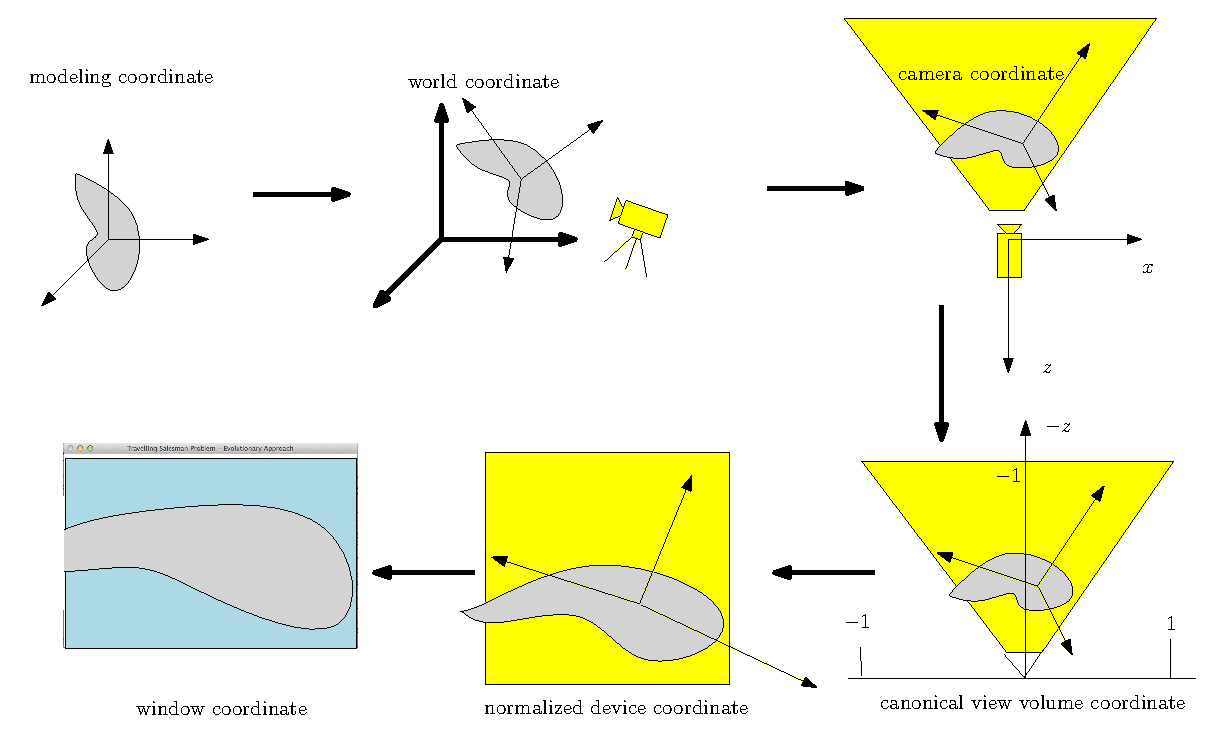
\includegraphics[height=6cm]{OGL_camera/coordinatesInPipeline.eps}
\end{figure}

\end{frame}
%%%%%%%%%%%%%%%%%%%%%%%%%%%%%%%%%%%%%%%%%%%%%%%%%%%%%%%%%

%%%%%%%%%%%%%%%%%%%%%%%%%%%%%%%%%%%%%%%%%%%%%%%%%%%%%%%%%
\begin{frame}{카메라 좌표 2/2}

\begin{itemize}
\item 모델링 좌표계를 기준으로 객체를 구성하는 각 정점의 좌표 결정
\item 객체에 적용되는 각종 변환들에 의해 전역 좌표(world coodinate)가 결정
\item 렌더링 파이프라인은 이를 화면에 출력하기 위해 카메라 좌표계로 변경
	\begin{itemize}
	\item 카메라의 위치가 원점이 되고, 카메라는 $z$축 음의 방향을 향함
	\end{itemize}
\item 관측볼륨의 변환
	\begin{itemize}
	\item 관측 볼륨 밖은 처리에서 제외
	\item 관측 볼륨은 클리핑 등이 효율적으로 이루어질 수 있는 표준 관측 볼륨(canonical viewing volume)으로 변환
	\item 표준 관측 볼륨은 정규 장치 좌표계로 변경: $x, y, z$의 범위가 모두 $[-1,1]$인 정육면체 공간
	\end{itemize}
\item 투영: 정규 장치 좌표에서 $z$ 값을 버리고 $(x,y)$만 취함
\end{itemize}

\end{frame}
%%%%%%%%%%%%%%%%%%%%%%%%%%%%%%%%%%%%%%%%%%%%%%%%%%%%%%%%%

%%%%%%%%%%%%%%%%%%%%%%%%%%%%%%%%%%%%%%%%%%%%%%%%%%%%%%%%%
\begin{frame}{카메라 기본 개념}

{\small
\begin{itemize}
\item 디폴트 카메라의 경우 중심이 원점이고, 각 변의 길이가 2인 상자 모양인데, 이 위치와 길이를 변경할 수 있다. 이를 지원하는 함수는 {\sf glOrtho}
\item glOrtho(float left, float right, float bottom, float top, float near, float far);
\end{itemize}
}

\begin{figure}
    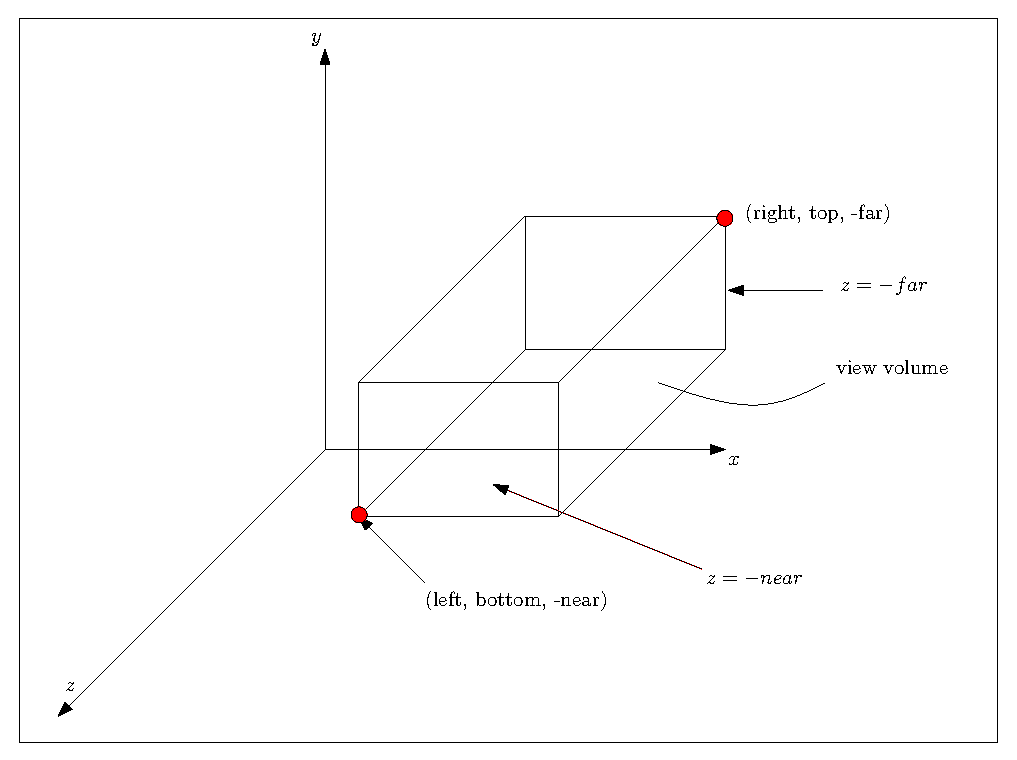
\includegraphics[height=6cm]{OGL_camera/cameraViewVolume.eps}
\end{figure}

\end{frame}
%%%%%%%%%%%%%%%%%%%%%%%%%%%%%%%%%%%%%%%%%%%%%%%%%%%%%%%%%

%%%%%%%%%%%%%%%%%%%%%%%%%%%%%%%%%%%%%%%%%%%%%%%%%%%%%%%%%
\begin{frame}{카메라 기본 개념}

{\small
\begin{itemize}
\item 디폴트 카메라의 경우 중심이 원점이고, 각 변의 길이가 2인 상자 모양인데, 이 위치와 길이를 변경할 수 있다. 이를 지원하는 함수는 {\sf glOrtho}
\item glOrtho(float left, float right, float bottom, float top, float near, float far);
\end{itemize}
}

\begin{figure}
    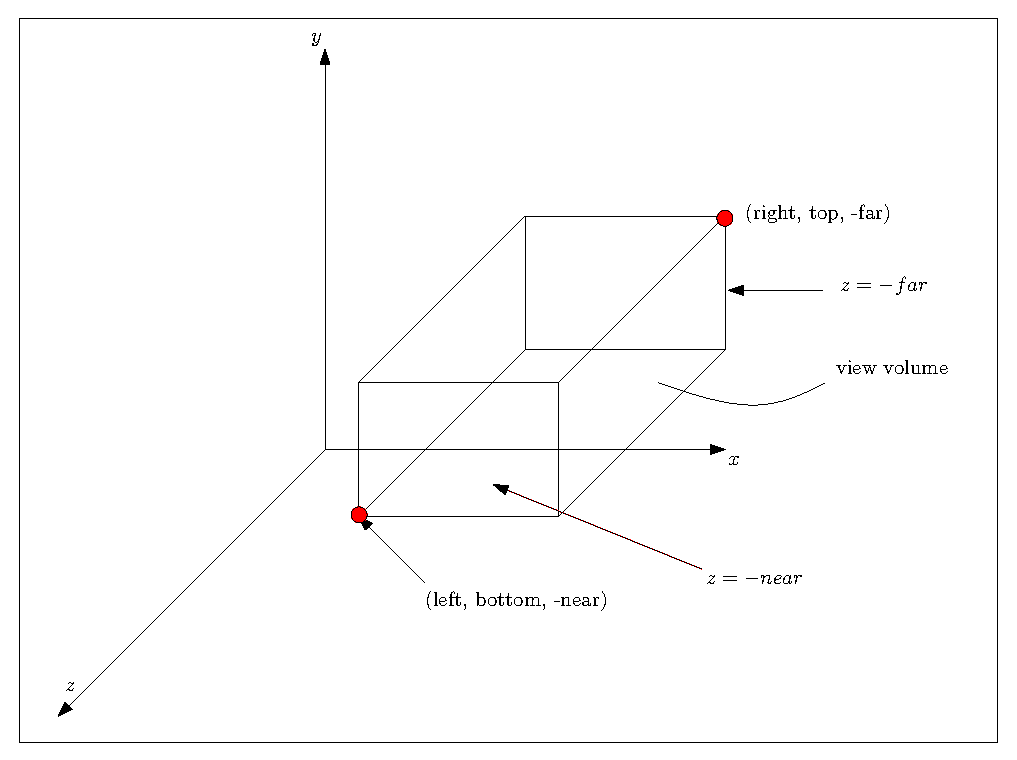
\includegraphics[height=6cm]{OGL_camera/cameraViewVolume.eps}
\end{figure}

\end{frame}
%%%%%%%%%%%%%%%%%%%%%%%%%%%%%%%%%%%%%%%%%%%%%%%%%%%%%%%%%

\end{document}



\chapter{카메라(Camera)}
\index{camera}






\section{OpenGL 카메라의 기본 개념}


각각의 파라미터가 가진 의미는 그림 \ref{fig:OGL_camera:cameraViewVolume}과 같다. 
이 파라미터들은 관측되는 공간의 크기를 결정하는데, {\sf left, right}는 $x$ 축 방향으로의 범위,
{\sf bottom, top}은 $y$ 축 방향으로의 범위를 표현한다.
그리고 {\sf near}와 {\sf far}는 클리핑(clipping) 평면을 결정하는데, 
가까운 쪽 클리핑 평면의 좌측 아래쪽 끝점이 ({\sf left, bottom, -near})이며,
먼 쪽 클리핑 평면의 우측 위쪽 끝점이 ({\sf right, top, -far})이다.
만약 {\sf near}가 음수 값이 주어지면 가까운 쪽 클리핑 평면이 관찰자의 등 뒤에 있다는 것을 의미한다.

\begin{verbatim}
glOrtho(-1,1, -1,1, -1,1);
\end{verbatim}

OpenGL은 그림 \ref{fig:OGL_camera:cameraViewVolume}의 관측공간(view volume)을 최초의 디폴트 카메라 공간으로 옮기는 변환을 수행한다. 
즉 관측공간 내부의 모든 객체가 디폴트 관측 공간인 (-1,1)$\times$(-1,1)$\times$(-1,1)로 옮겨지도록 하는 것이다. 
이 디폴트 관측 공간을 ‘정규 관측 공간(canonical view volume)‘이라 부른다. 
이러한 변환은 관측공간의 크기를 정규 관측 공간의 크기로 변경하고 중심을 원점으로 옮기는 것이다.
따라서 $x$ 축으로는 범위 $[left, right]$를 $[-1, 1]$로 변경하는 것이므로
그림 \ref{fig:OGL_camera:glOrthoXProjection}와 같은 직선으로 표현할 수 있다. 이는 다음과 같은 식으로 표현할 수 있다.

\begin{eqnarray}
\label{eq:OGL_camera:orthoXProjection}
x' = \left ( \frac{2}{right-left} \right ) x - \frac{right+left}{right-left}
\end{eqnarray}

\begin{figure}[h!]
  \centering
    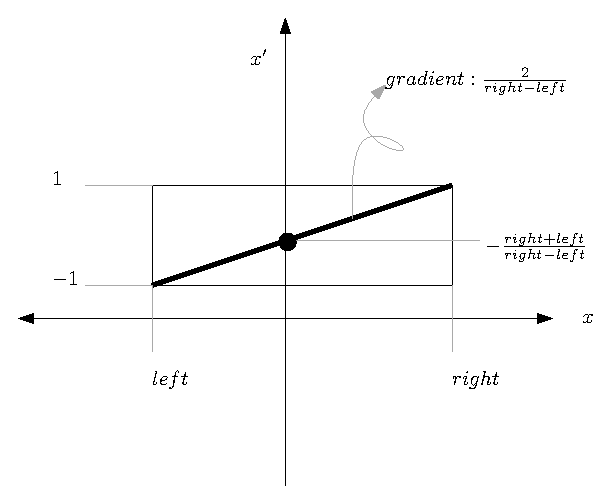
\includegraphics[height=8cm]{OGL_camera/glOrthoXProjection.eps}
    \caption{glOrtho 투영에 의한 $x$ 좌표의 변경}
    \label{fig:OGL_camera:glOrthoXProjection}
\end{figure}

비슷한 방법으로 $y$ 축 좌표의 변경도 가능하다. 이것은 다음과 같은 식으로 표현된다.

\begin{eqnarray}
\label{eq:OGL_camera:orthoYProjection}
y' = \left ( \frac{2}{top-bottom} \right ) y - \frac{top+bottom}{top-bottom}
\end{eqnarray}

$z$ 축 좌표는 부호가 바꾸어 적용되기 때문에 다음과 같이 표현할 수 있다.

\begin{eqnarray}
\label{eq:OGL_camera:orthoZProjection}
z' = - \left ( \frac{2}{far-near} \right ) z - \frac{far+near}{far-near}
\end{eqnarray}

그러므로 이러한 변환은 식 \ref{eq:OGL_camera:ortho_camera}와 같이 구할 수 있다.

\begin{eqnarray}
\left ( 
\begin{array}{cccc}
\frac{2}{right-left}& 0 & 0 & - \frac{right+left}{right-left}\\
0& \frac{2}{top-bottom} & 0 & - \frac{top+bottom}{top-bottom}\\
0& 0 & \frac{2}{far-near} & - \frac{far+near}{far-near}\\
0& 0 & 0 & 1
\end{array} 
\right )
\label{eq:OGL_camera:ortho_camera}
\end{eqnarray}


\subsection{원근 투영 카메라}
\index{원근 투영}\index{perspective camera}
실제 카메라나 우리 눈에는 멀리 있는 것은 작게 보이고 가까이 있는 것은 크게 보인다. 
그 이유는 빛이 관측 지점으로 모이면서 형성되는 선을 따라 원근투영되기 때문이다. 
이러한 원근 투영을 설정하는 방법은 {\sf glFrustum}과 {\sf gluPerspective}가 있다. 
우선 직관적인 다음의 {\sf gluPerspective} 함수를 이미 살펴 본 적이 있다.


\begin{figure}[h!]
  \centering
    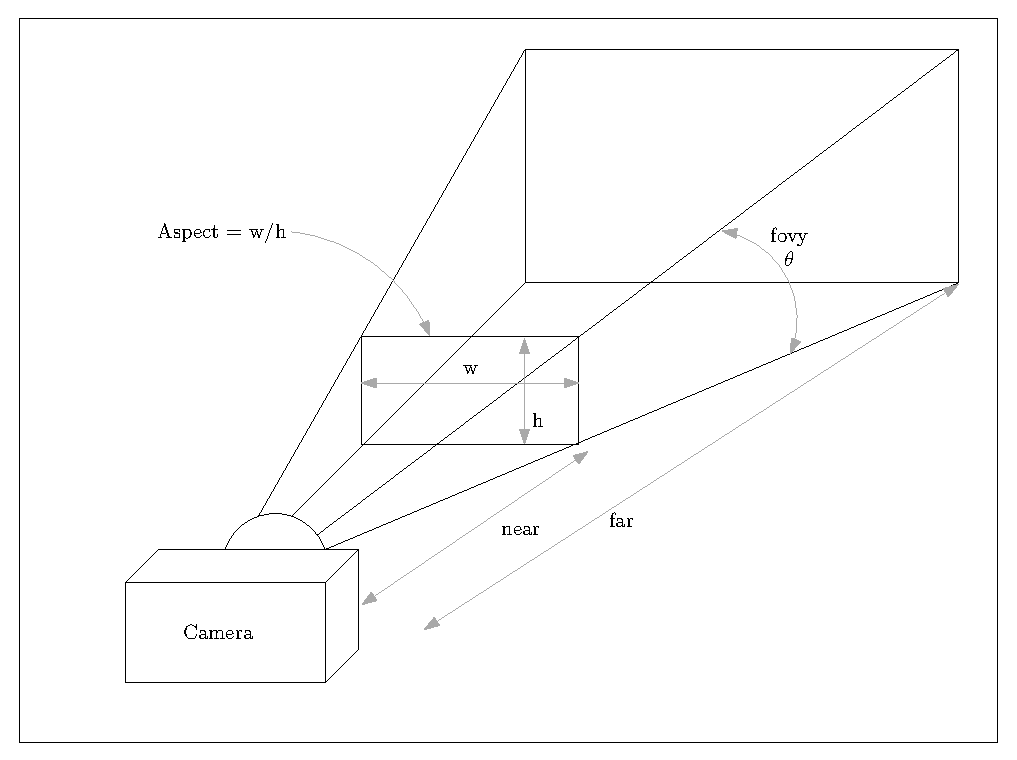
\includegraphics[height=8cm]{OGL_camera/perspectiveCam.eps}
    \caption{gluPerspective 파라미터의 의미}
    \label{fig:OGL_camera:perspectiveCam}
\end{figure}

\begin{verbatim}
gluPerspective(float fovy, float Aspect, float near, float far);
\end{verbatim}

이때 사용된 파라미터들의 의미는 그림 \ref{fig:OGL_camera:perspectiveCam}과 같다.

{\sf fovy}는 y축 방향으로의 시야각을 도(degree)로 나타낸 것이며, {\sf Aspect}는 가시화 볼륨의 종횡비(aspect ratio)를 의미하며, {\sf near}는 카메라에서 상이 맺히는 가까운 평면까지의 거리이며, {\sf far}는 가시화가 이루어지는 공간을 결정하는 평면 중 카메라에서 가장 먼 쪽 평면과 카메라 사이의 거리이다.
이 함수는 투영의 속성, 즉 카메라의 렌즈 속성을 결정한다. 따라서 이 함수는 그리기 동작이 일어날 때마다 불리는 것이 아니라 초기에 한 번, 혹은 렌즈를 바꿀 필요가 있을 때에만 불리게 된다.  {\sf glOrtho}를 통한 평행 투영과, gluPerspective를 통한 원근 투영은 그림 \ref{fig:OGL_camera:perspectiveCam}과 같이 상이 맺히는 것이다.


\begin{figure}[h!]
  \centering
    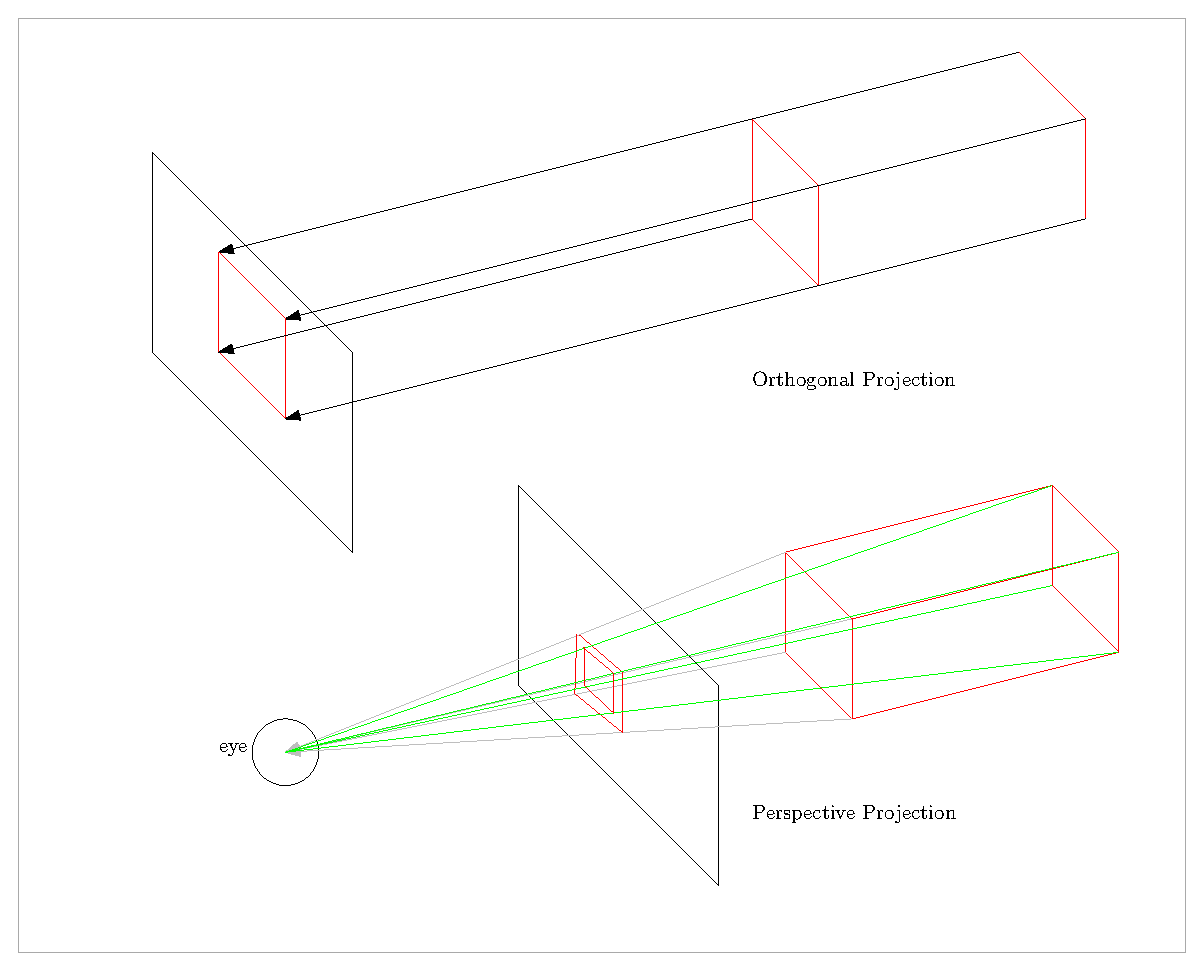
\includegraphics[height=8cm]{OGL_camera/projection.eps}
    \caption{직교 투영과 원근 투영의 비교}
    \label{fig:OGL_camera:perspectiveCam}
\end{figure}

\subsection{절단 공간}
3차원 그래픽스에서 사용하는 표준적인 카메라 모델은 렌더링의 대상이 되는 영역을 일정한 범위로 제한한다.
평행 투영(orthographic projection)을 수행할 경우 이 절단 공가은 세 개의 평행한 면의 짝(pair)으로 표현되는 직육면체가 된다.
원근이 있는 투영의 경우에는 절두체(frustum) 모양을 이룬다. 이 절두체는 모두 그림 \ref{fig:OGL_camera:frustumConcept}와 같은 
표준 관측 볼륨으로 변환이 가능하다. 

\begin{figure}[h!]
  \centering
    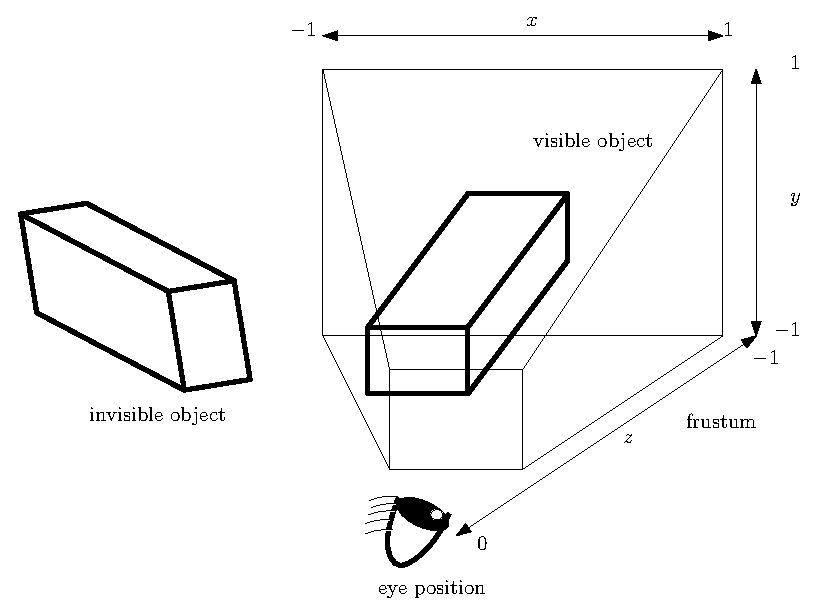
\includegraphics[height=9cm]{OGL_camera/frustumConcept.eps}
    \caption{표준 관측 볼륨(원근 투영의 예)}
    \label{fig:OGL_camera:frustumConcept}
\end{figure}

화면에 출력을 하기 위해서는 그림 \ref{fig:OGL_camera:frustumConcept}의 관측 볼륨을 그림 \ref{fig:OGL_camera:deviceCoordinate}의 정규 장치 좌표계로 바꾼다.

\begin{figure}[h!]
  \centering
    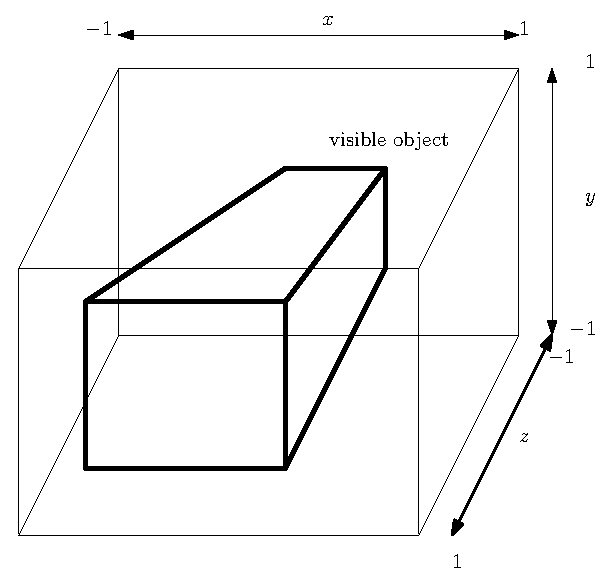
\includegraphics[height=8cm]{OGL_camera/deviceCoordinate.eps}
    \caption{정규 장치 좌표계}
    \label{fig:OGL_camera:deviceCoordinate}
\end{figure}

\section{카메라의 위치변경}

{\sf gluPerspective}를 사용하여도 카메라의 위치는 바뀌지 않는다. 즉 카메라는 여전히 원점 (0,0,0)에 놓여 있는 것이다. 카메라가 이렇게 고정되어 있으면 사물을 제대로 관찰할 수 없다. 이 카메라를 원하는 곳으로 옮겨주는 함수가 있는데 바로 {\sf gluLookAt}이다. 이 함수의 원형은 아래와 같다.

\begin{verbatim}
gluLookAt(
   float eye_x, float eye_y, float eye_z,
   float at_x, float at_y, float at_z,
   float up_x, float up_y, float up_z);
\end{verbatim}

\begin{figure}[h!]
  \centering
    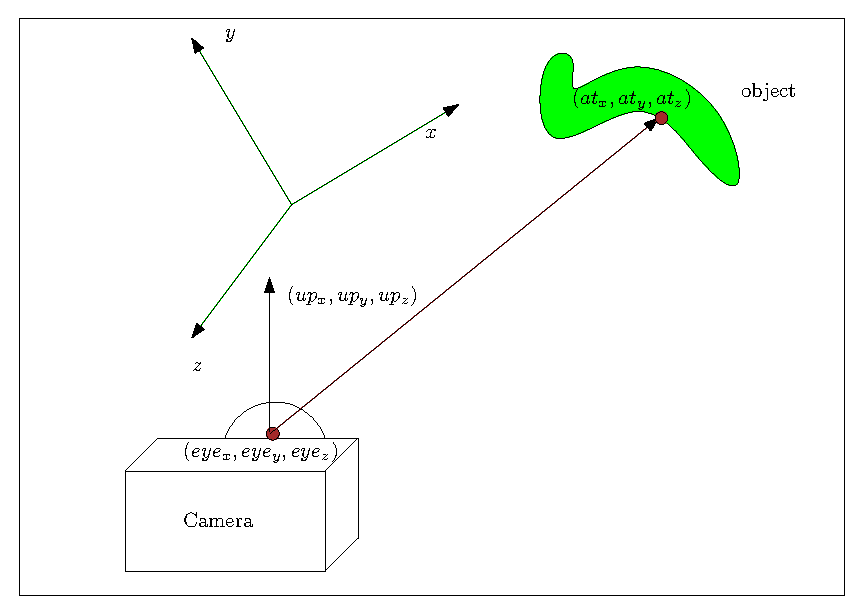
\includegraphics[height=8cm]{OGL_camera/cameraPositioning.eps}
    \caption{{\sf gluLookAt} 함수의 파라미터 이해}
    \label{fig:OGL_camera:gluLookAt}
\end{figure}

이때 사용되는 파라미터들의 의미는 그림 \ref{fig:OGL_camera:gluLookAt}과 같다.
이 함수는 투영의 속성을 바꾸는 것이 아니라 카메라를 옮겨 놓는 것인데, 실제 동작은 카메라 이동의 반대로 물체를 옮겨 놓는 것이다. 이 부분은 다음에 다시 자세히 다루기로 한다. 카메라의 위치는 매 프레임마다 변경될 수 있으므로 이 함수는 그리기 함수 내에서 매번 불리는 것이 일반적이다.

\subsection{행렬모드(Matrix mode)}\index{행렬 모드}\index{matrix mode}
OpenGL은 세 종류의 행렬을 가지고 있다. 텍스처 행렬, 모델뷰 행렬, 투영행렬이다. 이 가운데 가상공간 내의 좌표를 결정하는 행렬은 모델뷰 행렬과 투영행렬이다. 
모델뷰행렬(modelview matrix)은 공간 내에서 가상 객체를 변환하여 좌표를 변경하는 데에 사용되는 행렬이며, 투영행렬(projection matrix)은 가상 객체를 투영면에 옮겨 놓는 데에 사용되는 행렬이다. {\sf gluPerspective} 함수는 투영의 특성을 변경하는 것이므로 투영행렬 모드에서 동작한다. 반면 {\sf gluLookAt}은 투영의 특성이 아니라 카메라의 위치를 옮기는 것이고, 이는 바꾸어 말해 물체의 위치를 카메라 기준에서 옮기는 것이므로 모델뷰 행렬을 변경하는 것이다. 따라서 이 함수들은 각각 적절한 행렬 모드에서 동작해야 하며 다음과 같은 방식으로 프로그램에 포함된다.


\begin{verbatim}
glMatrixMode(GL_PROJECTION);
glLoadIdentity();
gluPerspective(60, 1.0, 0.1, 100.0);
//glOrtho(-1,1,-1,1,-1,1);
//glFrustum(-1,1,-1,1,1,10);
glMatrixMode(GL_MODELVIEW);
glLoadIdentity();
gluLookAt(1.0,1.0,1.0, 0.0, 0.0, 0.0, 0.0, 1.0, 0.0);
\end{verbatim}


\subsection{glFrustum}\index{glFrustum}
앞서는 이해를 쉽게 하기 위해 {\sf gluPerspective}를 사용하였지만 OpenGL에서 카메라의 원근 투영을 설정하는 가장 기본적인 방법은 
{\sf glFrustum} 함수를 이용하는 것이다.
{\sf glFrustum}은 {\sf glOrtho}와 동일한 파라미터를 가진다. 즉 다음과 같은 파라미터들을 받고, 그 아래의 그림과 같이 투영을 한다.

\begin{verbatim}
glFrustum(float left, float right,
          float bottom, float top, 
          float near, float far);
\end{verbatim}


\begin{figure}[h!]
  \centering
    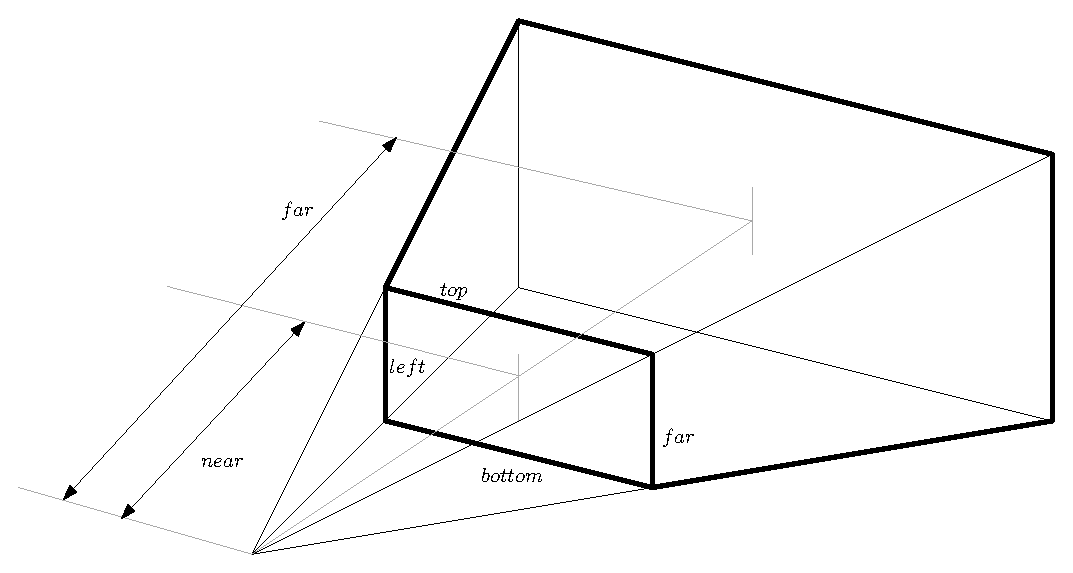
\includegraphics[height=7cm]{OGL_camera/glFrustum.eps}
    \caption{glFrustum 파라미터의 의미}
    \label{fig:OGL_camera:glFrustum}
\end{figure}

\index{glFrustum}
glFrustum은 원근 투영행렬을 생성하여 이 행렬을 현재의 투영행렬에 곱하는 작업을 수행한다. 곱의 결과가 새로운 투영행렬이 된다. 
따라서 일반적으로 사용되는 방법은 다음과 같다.
\begin{verbatim}
glMatrixMode(GL_PROJECTION);
glLoadIdentity();
glFrustum(l,r,b,t,n,f);
\end{verbatim}

\index{시야절두체}\index{view frustum}
위의 코드는 투영행렬을 우선 항등행렬 $\mathbf I$로 만든 뒤에 glFrustum이 표현하는 행렬을 곱하는 것이다.
그렇다면 이 glFrustum은 어떤 행렬을 생성할까? glFrustum은 시야절두체(view frustum)을 디폴트 카메라가 담는 공간, 즉 (-1,1)$\times$(-1,1)$\times$(-1,1)의 정규 관측 공간(canonical view cube)으로 변환시키는 행렬을 생성한다. 이 행렬은 우선 glFrustum으로 결정되는 절두체(frustum) 관측 공간을 glOrtho와 같은 평행 육면체로 변경한다. 그리고 나서 glOrtho의 투영행렬을 다시 적용하면 된다. glFrustum 공간을 평행 투영 공간으로 바꾸기 위해서는 다음 식 \ref{eq:OGL_camera:glFrustum}과 같은 변환이 필요하다. 이 식이 어떻게 유도되는지 살펴볼 것이다.

\begin{eqnarray}
\label{eq:OGL_camera:glFrustumMatrix}
\left ( 
\begin{array}{cccc}
\frac{2 near}{right-left}& 0 & \frac{right+left}{right - left} & 0\\
0& \frac{2 near}{top-bottom} & \frac{top+bottom}{top - bottom} & 0\\
0& 0 & -\frac{far+near}{far-near} & \frac{-2 near \cdot far}{far-near}\\
0& 0 & -1 & 0
\end{array} 
\right )
\label{eq:OGL_camera:glFrustum}
\end{eqnarray}

\subsection{glFrustum에 의한 투영행렬 구하기}

{\sf glFrustum}을 적용하면 위의 행렬과 같은 투영행렬이 생성되어 현재의 투영행렬에 곱해진다. 식 \ref{eq:OGL_camera:glFrustum}의 투영행렬은 
어떻게 구해진 것인지 살펴보자.

\index{근거리 클리핑 평면}\index{near clipping plane}
투영행렬을 구하는 것은 기본적으로 {\sf glFrustum}에 의해 결정되는 관측 볼륨(viewing volume)을 디폴트 카메라가 표현하는 것과 
같은 정규 관측 볼륨으로 변형하는 변환이다. 
그림 \ref{fig:OGL_camera:glFrustumXProjection}을 살펴보자.
그림에서 우선 {\sf glFrustum}이 담는 관측 볼륨 안의 어떤 점 $\mathbf p$의 동차좌표계 좌표를 $(p_x, p_y, p_z, 1)$이다.
이 점이 투영되어 가까운 쪽 클리핑 평면인 $z=-near$ 평면에 떨어진 지점의 좌표가 $(x,y,z,1)$이다.

\begin{figure}[h!]
  \centering
    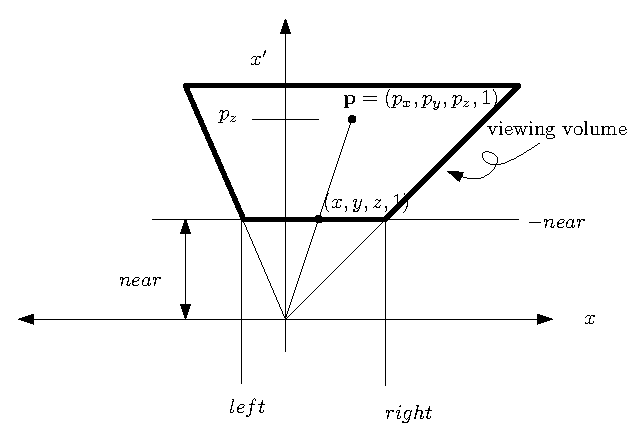
\includegraphics[height=8cm]{OGL_camera/glFrustumXProjection.eps}
    \caption{glFrustum의 투영}
    \label{fig:OGL_camera:glFrustumXProjection}
\end{figure}

닮은꼴 삼각형 사이의 비례를 이용하여 우리는 쉽게 
$p_x:p_z = x:-near$임을 알 수 있고, 다음과 같은 식을 유도할 수 있다.

\begin{eqnarray}
x = - near \frac{p_x}{p_z}
\end{eqnarray}

이렇게 해서 얻는 $x$ 좌표를 직교 투영에서 살펴본 바와 같이
식 \ref{eq:OGL_camera:orthoXProjection}를 이용하여 정규 장치 좌표계, 즉 $[-1,1]$의 범위로 옮겨 놓아야 한다.
이는 식 \ref{eq:OGL_camera:orthoXProjection}를 이용하여 다음과 같이 쉽게 구할 수 있다.

\begin{eqnarray}
\label{eq:OGL_camera:frustumXProjection}
x' = \left ( - \frac{2 near}{right-left} \right ) \frac{p_x}{p_z} - \frac{right+left}{right-left}
\end{eqnarray}

비슷한 방법으로 $y$ 좌표를 구하고 이를 정규 장치 좌표계의 좌표 $y'$로 바꾸는 작업도 다음과 같이 수행할 수 있다.

\begin{eqnarray}
\label{eq:OGL_camera:frustumYProjection}
y' = \left ( - \frac{2 near}{top-bottom} \right ) \frac{p_y}{p_z} - \frac{top + bottom}{top - bottom}
\end{eqnarray}

그런데, $z$ 좌표의 투영은 다소 고민을 해야 한다.
식 \ref{eq:OGL_camera:frustumXProjection}와 \ref{eq:OGL_camera:frustumYProjection}를 보면,
원래의 좌표 $p_x$와 $p_z$를 $p_z$로 나누는 작업을 포함하고 있다.
이러한 꼴을 표현하기 위해 $z$ 좌표의 변환도 이러한 꼴을 가질 수 있도록 다음과 같이 미지수 $\alpha$와 $\beta$를 포함한
1차식을 두자.

$$z' = \frac{\alpha}{p_z} + \beta$$

이 식은 $p_z$가 $near$인 경우에는 -1, $far$인 경우에는 $1$의 값을 가져야 한다. 그러므로, 우리는 미지수를 알아낼 수 있는 다음 두
식을 얻게 된다.

\begin{eqnarray}
\label{eq:OGL_camera:frustumZProjectionPre}
-1 & = & \frac{\alpha}{near} + \beta \\ \nonumber
  1 & = & \frac{\alpha}{far} + \beta
\end{eqnarray}

이 이원일차연립방정식을 풀면 $\alpha$와 $\beta$를 다음과 같이 구할 수 있다.

$$\alpha = \frac{near \cdot far}{far - near}, ~~~ \beta = \frac{far+near}{far-near}$$

이제 정규 장치 좌표계 내의 좌표 ${\mathbf p}'(x',y',z',1)$은 다음과 같이 ${\mathbf p}(p_x, p_y, p_z, 1)$을 이용하여
표현할 수 있다.
\begin{eqnarray}
\left (
\begin{array}{c}
x\\
y\\
z\\
1
\end{array} 
\right ) =
\left ( 
\begin{array}{c}
-x \cdot p_x\\
-y \cdot p_y\\
-z \cdot p_z\\
-p_z
\end{array} 
\right )=
\left ( 
\begin{array}{cccc}
\frac{2 near}{right - left} p_x + \frac{right+left}{right-left} p_z \\
\frac{2 near}{top - bottom} p_y + \frac{top+bottom}{top-bottom} p_z \\
-\frac{far + near}{right - left} p_z - \frac{2 near \cdot far}{far - near} \\
- p_z \\
\end{array}
\right )
\end{eqnarray}

이상의 결과를 통해 우리는 {\sf glFrustum}에 의해 만들어지는 투영행렬이 
식 \ref{eq:OGL_camera:glFrustumMatrix}과 같음을 알 수 있다.
여기서 {\sf far}의 값이 무한대인 경우, 즉, 먼쪽 클리핑 평면이 없는 경우의 투영행렬이 어떻게 될지 고민해 보라.

%%%%%%%%%%%%%%%%%%


우리는 앞서 직관적 이해가 쉬운 gluPerspective를 사용하였다. 그러나 내부적으로 이 함수는 glFrustum을 호출하게 되어 있다. gluPerspective에 사용된 파라미터를 이용하여 glFrustum 함수에 적용되는 파라미터를 계산할 수 있는데, 이 둘은 다음 관계를 갖는다.

\begin{verbatim}
gluPerspective(fovy, aspect, near, far);
glFrustum(left,right,bottom,top,near,far);
\end{verbatim}

$$top = near \cdot \tan \frac{\theta}{2}$$
$$bottom = -near \cdot \tan \frac{\theta}{2}$$
$$right = top \cdot aspect$$
$$left = bottom \cdot aspect$$

\section{오픈지엘(OpenGL) 카메라의 특성 제어}\index{카메라!오픈지엘 카메라}\index{OpenGL!camera}

이제 지금까지 사용한 간단한 카메라를 조금 더 유용하게 개선하여 보자. 우선 지금까지의 카메라는 다음과 같은 심각한 문제를 가지고 있다.
카메라의 종횡비가 1이어서 창의 크기를 변경하면 그려지는 결과에 왜곡이 발생한다. 즉 그림 \ref{fig:OGL_camera:aspectRatioDistort}과 같이 정사각형 창의 경우에는 제대로 그려지지만, 상하로 긴 창에서는 주전자도 함께 길어진다. 창이 좌우로 길어져도 비슷한 왜곡이 발생한다.

\begin{figure}[h!]
  \centering
    \fbox{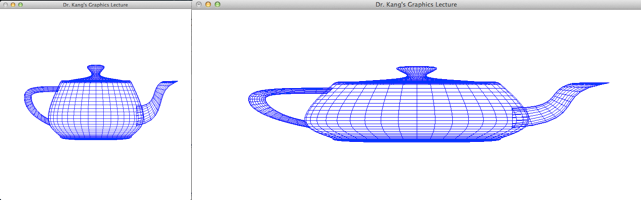
\includegraphics[height=4cm]{OGL_camera/aspectRatioDistort.png}}
    \caption{종횡비(aspect ratio)에 따라 왜곡되는 화면}
    \label{fig:OGL_camera:aspectRatioDistort}
\end{figure}

창 크기가 변경되는 이벤트의 처리 함수는 GLUT의 API를 이용하여 {\sf glutReshapeFunc} 함수로 등록할 수 있다. 이때 등록되는 콜백(callback) 함수는 다음의 프로토타입(prototype)을 갖는다.

\begin{verbatim}
void reshapeFunction(int w, int h);
\end{verbatim}

여기에서 {\sf w}와 {\sf h}는 새롭게 변경된 창의 가로와 세로 픽셀 수이다. 이를 이용하여 코드 \ref{code:OGL_camera:reshapeWindow}과 같이 
{\sf glOrtho}를 설정하면 그림 \ref{fig:OGL_camera:aspectRatioNoDistort}에서 확인할 수 있는 바와 같이 왜곡없는 카메라를 구현할 수 있다.



\begin{algorithmbis}[창 크기 변경에 따른 카메라 재설정]\label{code:OGL_camera:reshapeWindow}
\lstset{language=C++, escapechar=^} 
\begin{lstlisting}
^{\sf [[헤더 파일 포함하기]]^

void init(int argc, char **argv) {
   ^{\sf [[윈도우, 버퍼 초기화 작업]]^

   glMatrixMode(GL_PROJECTION);
   glLoadIdentity();
   glOrtho(-2.0, 2.0, -2.0, 2.0, -2.0, 2.0);
}
void reshape(int w, int h) {
   float asp = float(w)/float(h);
   glViewport(0, 0, w, h);
   glMatrixMode(GL_PROJECTION);
   glLoadIdentity();
   glOrtho(-2.0*asp, 2.0*asp,    -2.0, 2.0,  -2.0, 2.0);
   glutPostRedisplay();
}
void display() {
   glClear(GL_COLOR_BUFFER_BIT);
   glMatrixMode(GL_MODELVIEW);
   glLoadIdentity();
   glutWireTeapot(1.0);
   glutSwapBuffers();
}
int main(int argc, char **argv) {
   init(argc, argv);
   glutDisplayFunc(display);
   glutReshapeFunc(reshape);
   glutMainLoop();
}
\end{lstlisting}
\end{algorithmbis}


\begin{figure}[h!]
  \centering
    \fbox{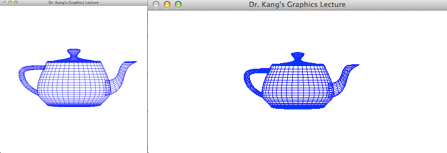
\includegraphics[height=4cm]{OGL_camera/aspectRatioNoDistort.png}}
    \caption{종횡비(aspect ratio)가 달라도 왜곡되지 않는 화면}
    \label{fig:OGL_camera:aspectRatioNoDistort}
\end{figure}

{\sf gluPerspective}를 사용할 경우에는 더욱 간단하다. 이 함수의 두 번째 파라미터로 종횡비를 바로 입력하면 된다. 그러면 {\sf gluPerspective}는 
적절한 {\sf glFrustum}을 계산한다.
키보드 이벤트를 이용하여 카메라를 직교 카메라(orthographic camera)와 원근 카메라(perspective camera)로 변경할 수 있도록 할 것이며, 
카메라의 줌인(zoom-in), 줌아웃(zoom-out)도 가능하게 할 것이다.
우선 키보드를 처리하는 콜백함수의 등록을 한다. 이는 {\sf glutKeyboardFunc} 함수를 통해 가능하다. 
카메라의 종류는 {\sf bOrthoCam}이 결정한다. 이 값이 {\sf true}이면 
{\sf glOrtho}를 불러 직교 투영 카메라를 사용하고, {\sf false}이면 {\sf gluPerspective}를 불러 원근 투영 카메라를 사용한다. 
다음으로 줌인/줌아웃은 {\sf zoomFactor}라는 변수에 의해 결정된다. 이 값이 커지면 줌인, 작아지면 줌아웃이 되도록 할 것이다. 
이를 구현하기 위해서 {\sf glOrtho}와 {\sf glPerspective}에 실제로 적용하는 방식은 약간 다르다.

{\sf glOrtho}의 경우 줌인/줌아웃을 수행하기 위해서는 좌우, 상하의 값을 변경해야 한다. 이는 {\sf zoomFactor}로 이 값들을 나눠주면 된다. 

\begin{verbatim}
glOrtho(-2.0*aspRatio/zoomFactor, 2.0*aspRatio/zoomFactor, 
        -2.0/zoomFactor, 2.0/zoomFactor, 
        -200.0, 200.0);
\end{verbatim}


{\sf gluPerspective}는 첫 번째 파라미터가 시야각을 결정한다. 줌인이라는 것은 망원렌즈의 배율이 올라가는 것과 같고, 이는 투영의 각을 좁히는 것으로 흉내낼 수 있다. 따라서 {\sf zoomFactor}를 이용하여 이 {\sf fovy}, 즉 시야각을 나눠주면 된다.

\begin{verbatim}
gluPerspective(60/zoomFactor, aspRatio, 0.1, 100);
\end{verbatim}

또한 {\sf glOrtho}를 사용할 때에는 카메라가 원점에 있었도 문제가 없지만, {\sf gluPerspective}를 사용할 때에는 
카메라가 원점에 있으면 이 근처에 있는 주전자가 너무 크며, 일부 면을 볼 수 없다. 이를 해결하기 위해서는 카메라의 위치를 
{\sf gluLookAt}을 통해 관측가능한 곳으로 이동해 놓는다.
따라서 이 프로그램은 다음 코드 \ref{code:OGL_camera:cameraLensControl}과 같이 수정하여 ‘m’ 키에 의해 직교투영 카메라나 원근투영 카메라로 상호 변환될 수 있으며, ‘$<$‘ 키와 ‘$>$’를 이용하여 확대축소가 가능하다. 코드는 다음과 같이 정리된다.

\begin{algorithmbis}[카메라 렌즈 특성 선택 및 조작]\label{code:OGL_camera:cameraLensControl}
\lstset{language=C++, escapechar=^} 
\begin{lstlisting}
bool  bOrthoCam = true;
float aspRatio = 1.0;
float zoomFactor = 1.0;
void setCamera(void) {
   glMatrixMode(GL_PROJECTION);
   glLoadIdentity();
   if (bOrthoCam) {
      glOrtho(-2.0*aspRatio/zoomFactor, 
               2.0*aspRatio/zoomFactor, 
              -2.0/zoomFactor, 2.0/zoomFactor, 
              -200.0, 200.0);
   }
   else { // perspective camera
      gluPerspective(60/zoomFactor, aspRatio, 0.1, 100);
   }
}
void init(int argc, char **argv) {
   ^{\sf [[필요한 윈도우, 버퍼, 카메라 초기화 작업]]^
}
void keyboard(unsigned char k, int x, int y) {
   switch (k) {
      case 'm': bOrthoCam = bOrthoCam?false:true; break; // ^{\it 카메라 변경}^
      case '<': zoomFactor *= 0.95; break; // ^{\it 줌 아웃}^
      case '>': zoomFactor *= 1.05; break; // ^{\it 줌 인}^
      default: break;
   }
   setCamera();
   glutPostRedisplay();
}
void reshape(int w, int h) {
   aspRatio = float(w)/float(h);
   glViewport(0, 0, w, h);
   setCamera();
}
void display() {
   glClear(GL_COLOR_BUFFER_BIT);
   glMatrixMode(GL_MODELVIEW);
   glLoadIdentity();
   gluLookAt(0.0, 0.0, 3.0, 0.0, 0.0, 0.0, 0.0, 1.0, 0.0);
   glutWireTeapot(1.0);
   glutSwapBuffers();
}
int main(int argc, char **argv) {
   init(argc, argv);
   glutDisplayFunc(display);
   glutReshapeFunc(reshape);
   glutKeyboardFunc(keyboard);
   glutMainLoop();
}
\end{lstlisting}
\end{algorithmbis}

코드 \ref{code:OGL_camera:cameraLensControl}를 구현한 결과에서는 그림 \ref{fig:OGL_camera:cameraLensControl}와 같이 다양한 렌즈 특성을 테스트 할 수 있다.
\begin{figure}[h!]
  \centering
    \fbox{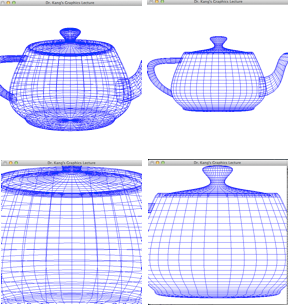
\includegraphics[height=4cm]{OGL_camera/cameraLensControl.png}}
    \caption{다양한 카메라 렌즈 특성을 설정한 결과}
    \label{fig:OGL_camera:cameraLensControl}
\end{figure}

카메라와 투영행렬에 대한 더 자세한 설명을 위해서는 \cite{lengyel2004mathematics,ryu20043d,dunn20113d} 등을 참고하라.

